\section{Introduction}
\label{industry_needs}
As we mentioned in chapter \ref{chapter_general_intro}, the aim of this thesis was twofold: deriving a methodology for inferring the motivational state of individuals while interacting with potentially rewarding object and presenting how this could be used in industry settings for automated engagement prediction.

In this chapter we will focus on sketching a system design for employing our methodology in an industry setting. First we will provide an overview of which potential need an industry player (or a collection of) might have with respect to engagement prediction. We will then proceed at illustrating a system designed for serving this needs. Finally we will present how the components of this system connect with the work we presented so far and how can be leveraged for satisfying said needs.

\section{The Needs from the Videogames Industry}
\label{industry_needs}
\lorem

\section{Multi-context Automated Engagement Prediction and Quantification}
\label{industry_needs}

\section{Data Generation}
\lorem
\section{Model Owner}
\lorem
\subsection{Data Storage}
\lorem
\subsection{Model Generation}
\lorem
\section{Model Consumer}
\lorem
\subsection{Representation Sharing}
\lorem
\subsection{Profile Generation}
\lorem
\subsection{Live Predictions}
\lorem
\subsection{Automated Reporting}
\lorem

\begin{figure}[ht]
\centering
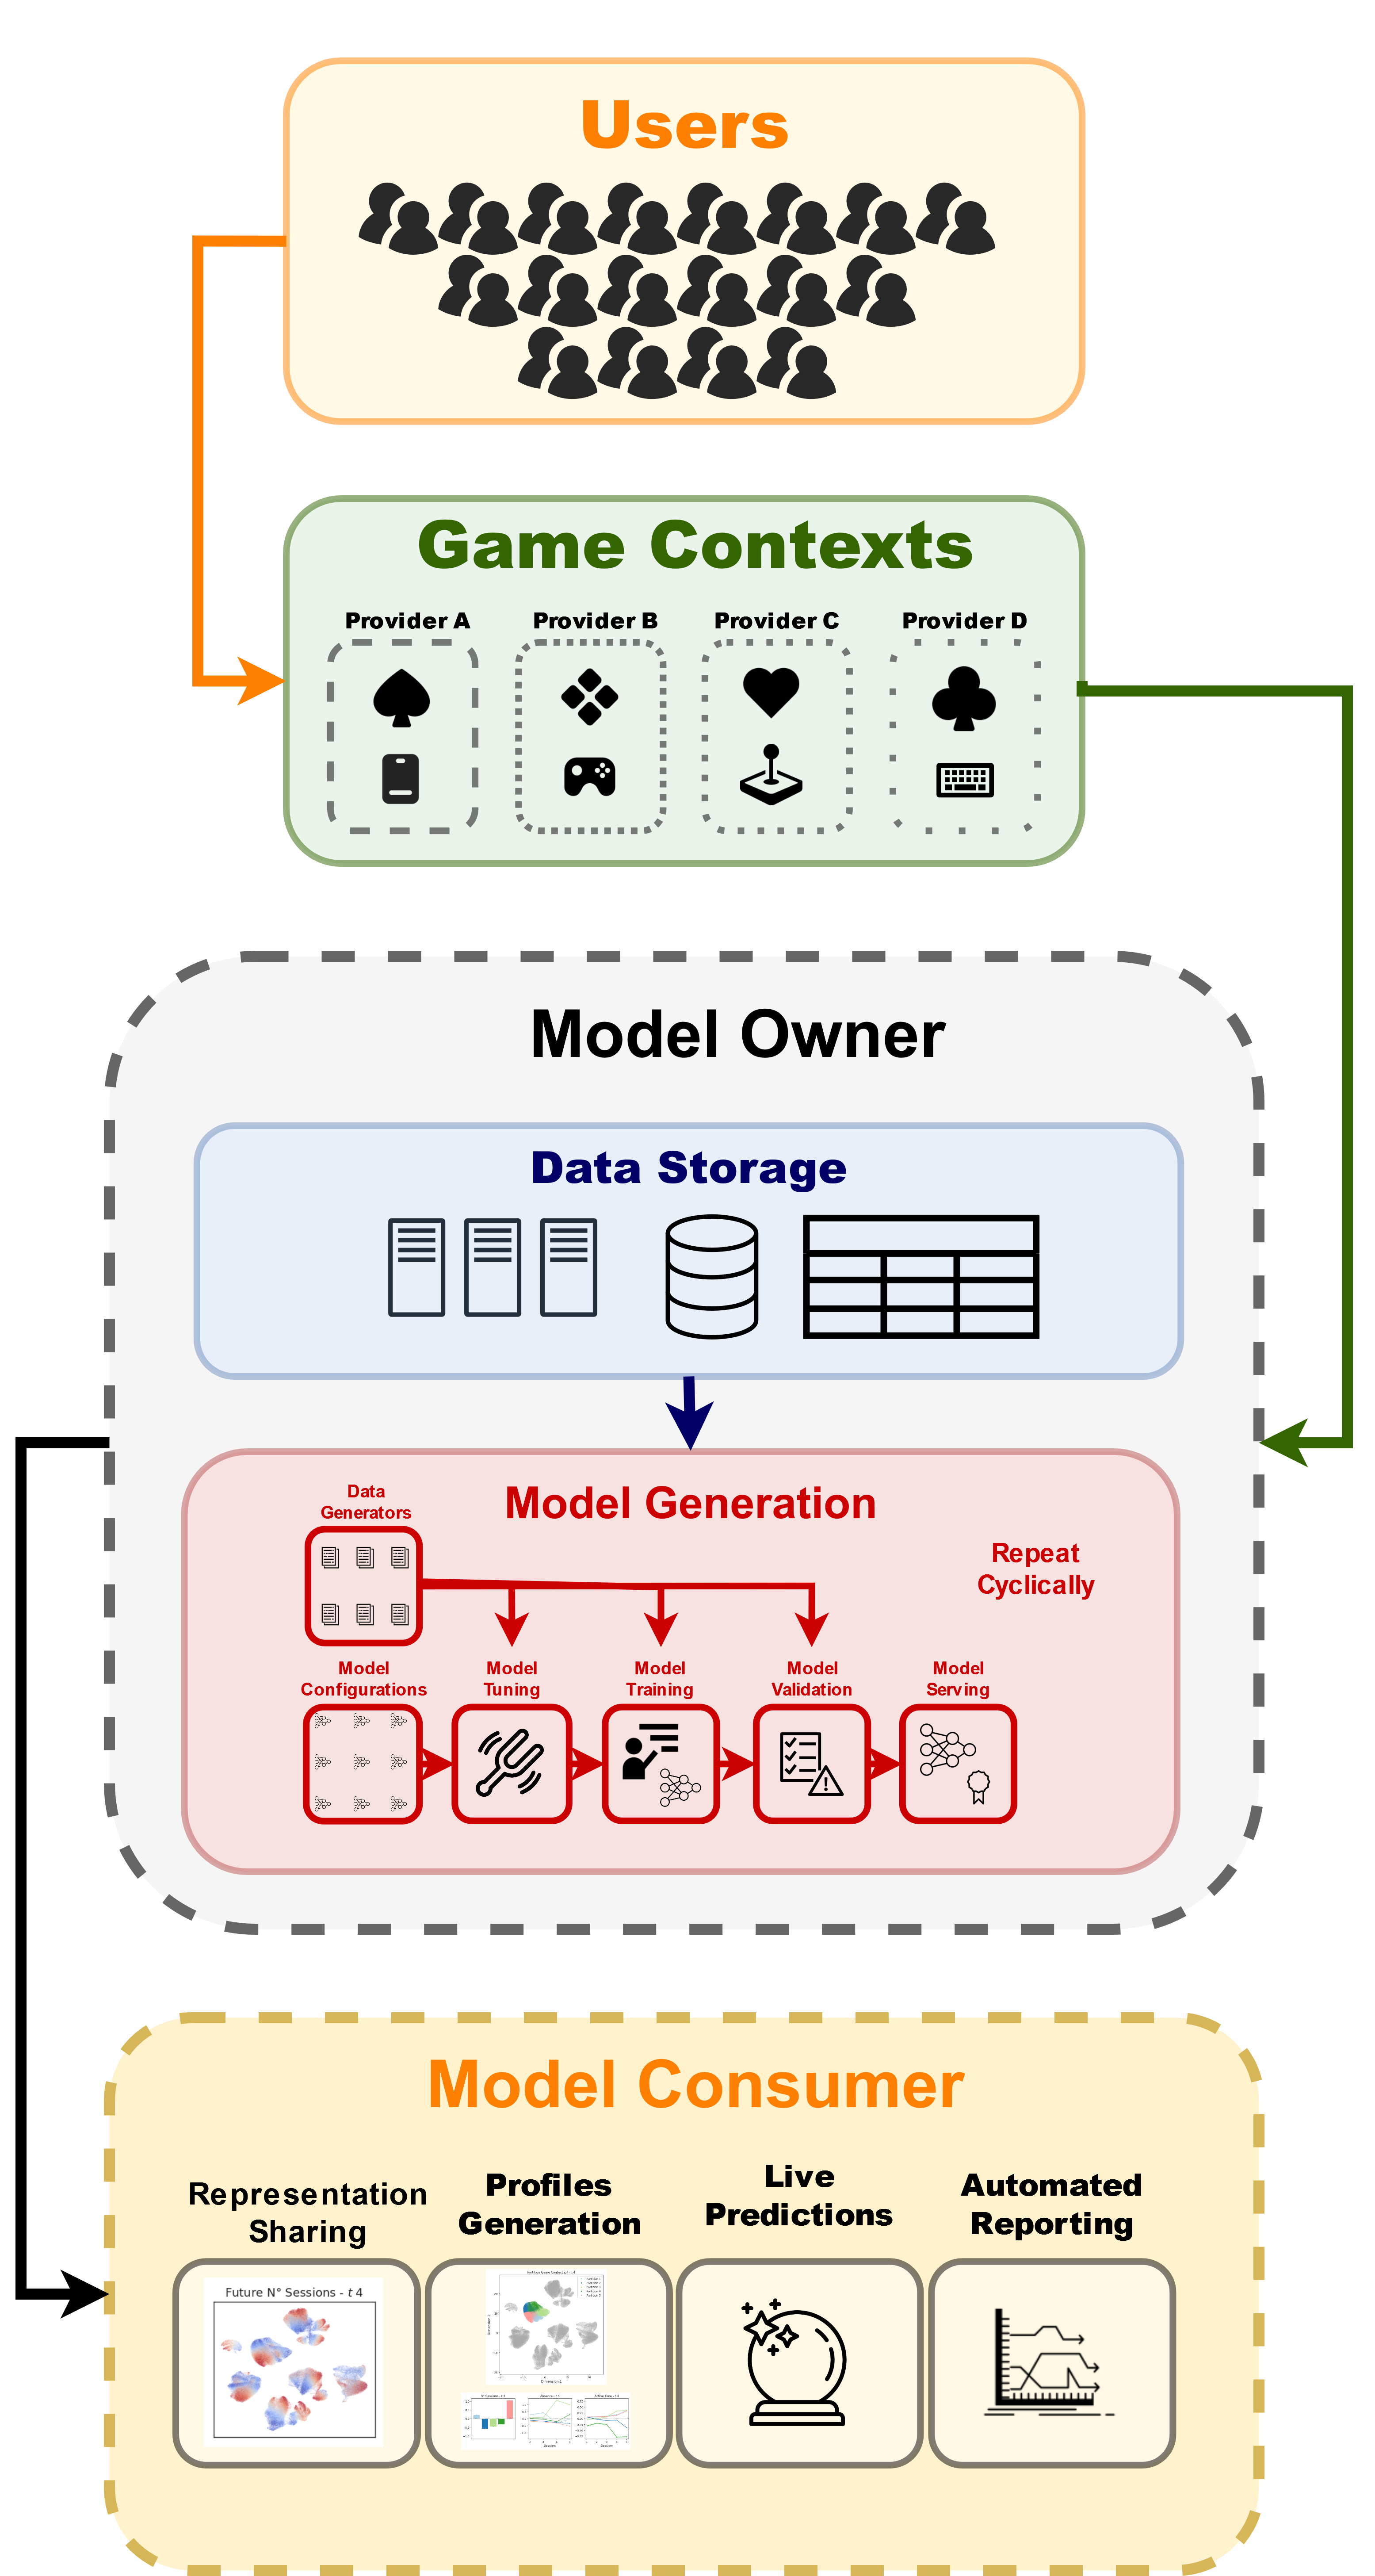
\includegraphics[width=0.7\textwidth]{images/chapter_5/pipeline_diagram.png}
\caption[\textbf{Model Deployment Pipeline}]{The figure represents a simplified system diagram for a potential application of the improved RNN architecture. Solid lines represent low-level components in the system while dashed lines indicate high-level entities. Directional arrows represent the flow of operations inside the system.}
\label{pipeline}
\end{figure}